\documentclass[twoside]{book}

% Packages required by doxygen
\usepackage{fixltx2e}
\usepackage{calc}
\usepackage{doxygen}
\usepackage{graphicx}
\usepackage[utf8]{inputenc}
\usepackage{makeidx}
\usepackage{multicol}
\usepackage{multirow}
\PassOptionsToPackage{warn}{textcomp}
\usepackage{textcomp}
\usepackage[nointegrals]{wasysym}
\usepackage[table]{xcolor}

% NLS support packages
\usepackage[french]{babel}

% Font selection
\usepackage[T1]{fontenc}
\usepackage{mathptmx}
\usepackage[scaled=.90]{helvet}
\usepackage{courier}
\usepackage{amssymb}
\usepackage{sectsty}
\renewcommand{\familydefault}{\sfdefault}
\allsectionsfont{%
  \fontseries{bc}\selectfont%
  \color{darkgray}%
}
\renewcommand{\DoxyLabelFont}{%
  \fontseries{bc}\selectfont%
  \color{darkgray}%
}
\newcommand{\+}{\discretionary{\mbox{\scriptsize$\hookleftarrow$}}{}{}}

% Page & text layout
\usepackage{geometry}
\geometry{%
  a4paper,%
  top=2.5cm,%
  bottom=2.5cm,%
  left=2.5cm,%
  right=2.5cm%
}
\tolerance=750
\hfuzz=15pt
\hbadness=750
\setlength{\emergencystretch}{15pt}
\setlength{\parindent}{0cm}
\setlength{\parskip}{0.2cm}
\makeatletter
\renewcommand{\paragraph}{%
  \@startsection{paragraph}{4}{0ex}{-1.0ex}{1.0ex}{%
    \normalfont\normalsize\bfseries\SS@parafont%
  }%
}
\renewcommand{\subparagraph}{%
  \@startsection{subparagraph}{5}{0ex}{-1.0ex}{1.0ex}{%
    \normalfont\normalsize\bfseries\SS@subparafont%
  }%
}
\makeatother

% Headers & footers
\usepackage{fancyhdr}
\pagestyle{fancyplain}
\fancyhead[LE]{\fancyplain{}{\bfseries\thepage}}
\fancyhead[CE]{\fancyplain{}{}}
\fancyhead[RE]{\fancyplain{}{\bfseries\leftmark}}
\fancyhead[LO]{\fancyplain{}{\bfseries\rightmark}}
\fancyhead[CO]{\fancyplain{}{}}
\fancyhead[RO]{\fancyplain{}{\bfseries\thepage}}
\fancyfoot[LE]{\fancyplain{}{}}
\fancyfoot[CE]{\fancyplain{}{}}
\fancyfoot[RE]{\fancyplain{}{\bfseries\scriptsize Généré le Vendredi 27 Mars 2015 12\+:15\+:26 pour C\+R\+T\+C par Doxygen }}
\fancyfoot[LO]{\fancyplain{}{\bfseries\scriptsize Généré le Vendredi 27 Mars 2015 12\+:15\+:26 pour C\+R\+T\+C par Doxygen }}
\fancyfoot[CO]{\fancyplain{}{}}
\fancyfoot[RO]{\fancyplain{}{}}
\renewcommand{\footrulewidth}{0.4pt}
\renewcommand{\chaptermark}[1]{%
  \markboth{#1}{}%
}
\renewcommand{\sectionmark}[1]{%
  \markright{\thesection\ #1}%
}

% Indices & bibliography
\usepackage{natbib}
\usepackage[titles]{tocloft}
\setcounter{tocdepth}{3}
\setcounter{secnumdepth}{5}
\makeindex

% Hyperlinks (required, but should be loaded last)
\usepackage{ifpdf}
\ifpdf
  \usepackage[pdftex,pagebackref=true]{hyperref}
\else
  \usepackage[ps2pdf,pagebackref=true]{hyperref}
\fi
\hypersetup{%
  colorlinks=true,%
  linkcolor=blue,%
  citecolor=blue,%
  unicode%
}

% Custom commands
\newcommand{\clearemptydoublepage}{%
  \newpage{\pagestyle{empty}\cleardoublepage}%
}


%===== C O N T E N T S =====

\begin{document}

% Titlepage & ToC
\hypersetup{pageanchor=false,
             bookmarks=true,
             bookmarksnumbered=true,
             pdfencoding=unicode
            }
\pagenumbering{roman}
\begin{titlepage}
\vspace*{7cm}
\begin{center}%
{\Large C\+R\+T\+C }\\
\vspace*{1cm}
{\large Généré par Doxygen 1.8.8}\\
\vspace*{0.5cm}
{\small Vendredi 27 Mars 2015 12:15:26}\\
\end{center}
\end{titlepage}
\clearemptydoublepage
\tableofcontents
\clearemptydoublepage
\pagenumbering{arabic}
\hypersetup{pageanchor=true}

%--- Begin generated contents ---
\chapter{Classe C\+I2\+C}
\label{index}\hypertarget{index}{}\begin{DoxyAuthor}{Auteur}
Simon Moinet 
\end{DoxyAuthor}
\begin{DoxyDate}{Date}
Mars 2015
\end{DoxyDate}
Cette classe \hyperlink{classCI2C}{C\+I2\+C} permet de lire/écrire les valeurs de registres des esclaves d'un bus I2\+C 
\chapter{Index hiérarchique}
\section{Hiérarchie des classes}
Cette liste d'héritage est classée approximativement par ordre alphabétique \+:\begin{DoxyCompactList}
\item \contentsline{section}{C\+I2\+C}{\pageref{class_c_i2_c}}{}
\item exception\begin{DoxyCompactList}
\item \contentsline{section}{C\+I2\+C\+:\+:Erreur}{\pageref{class_c_i2_c_1_1_erreur}}{}
\end{DoxyCompactList}
\end{DoxyCompactList}

\chapter{Index des classes}
\section{Liste des classes}
Liste des classes, structures, unions et interfaces avec une brève description \+:\begin{DoxyCompactList}
\item\contentsline{section}{\hyperlink{classCI2C}{C\+I2\+C} \\*Cette classe \hyperlink{classCI2C}{C\+I2\+C} permet de lire/écrire les valeurs de registres des esclaves d'un bus I2\+C }{\pageref{classCI2C}}{}
\item\contentsline{section}{\hyperlink{classCI2C_1_1ErreurDevNotDefine}{C\+I2\+C\+::\+Erreur\+Dev\+Not\+Define} \\*Exception device non défini }{\pageref{classCI2C_1_1ErreurDevNotDefine}}{}
\item\contentsline{section}{\hyperlink{classCI2C_1_1ErreurOpenDev}{C\+I2\+C\+::\+Erreur\+Open\+Dev} \\*Exception lorsqu'on essaye d'ouvrir le dev spécifié }{\pageref{classCI2C_1_1ErreurOpenDev}}{}
\item\contentsline{section}{\hyperlink{classCI2C_1_1ErreurRead}{C\+I2\+C\+::\+Erreur\+Read} \\*Cette classe est une exception qui est levé lorsqu'il y a un erreur de lecture }{\pageref{classCI2C_1_1ErreurRead}}{}
\item\contentsline{section}{\hyperlink{classCI2C_1_1ErreurSetAddrSlave}{C\+I2\+C\+::\+Erreur\+Set\+Addr\+Slave} \\*Exception definition de l'esclave }{\pageref{classCI2C_1_1ErreurSetAddrSlave}}{}
\item\contentsline{section}{\hyperlink{classCI2C_1_1ErreurSlaveNotDefine}{C\+I2\+C\+::\+Erreur\+Slave\+Not\+Define} \\*Exception adresse de l'esclave non défini }{\pageref{classCI2C_1_1ErreurSlaveNotDefine}}{}
\item\contentsline{section}{\hyperlink{classCI2C_1_1ErreurWrite}{C\+I2\+C\+::\+Erreur\+Write} \\*Cette classe est une esception qui est levé lorsqu'il y a une erreur d'écriture }{\pageref{classCI2C_1_1ErreurWrite}}{}
\end{DoxyCompactList}

\chapter{Index des fichiers}
\section{Liste des fichiers}
Liste de tous les fichiers avec une brève description \+:\begin{DoxyCompactList}
\item\contentsline{section}{/home/jam/\+Bureau/\+C++/\+Classes/\+C\+I2\+C/\hyperlink{_c_i2_c_8cpp}{C\+I2\+C.\+cpp} }{\pageref{_c_i2_c_8cpp}}{}
\item\contentsline{section}{/home/jam/\+Bureau/\+C++/\+Classes/\+C\+I2\+C/\hyperlink{_c_i2_c_8h}{C\+I2\+C.\+h} }{\pageref{_c_i2_c_8h}}{}
\end{DoxyCompactList}

\chapter{Documentation des classes}
\hypertarget{classCI2C}{\section{Référence de la classe C\+I2\+C}
\label{classCI2C}\index{C\+I2\+C@{C\+I2\+C}}
}


Cette classe \hyperlink{classCI2C}{C\+I2\+C} permet de lire/écrire les valeurs de registres des esclaves d'un bus I2\+C.  




{\ttfamily \#include $<$C\+I2\+C.\+h$>$}



Graphe de collaboration de C\+I2\+C\+:\nopagebreak
\begin{figure}[H]
\begin{center}
\leavevmode
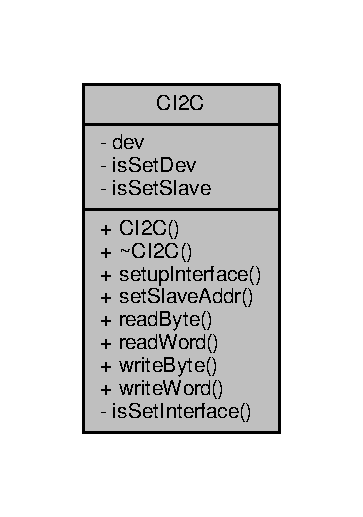
\includegraphics[width=174pt]{classCI2C__coll__graph}
\end{center}
\end{figure}
\subsection*{Classes}
\begin{DoxyCompactItemize}
\item 
class \hyperlink{classCI2C_1_1ErreurDevNotDefine}{Erreur\+Dev\+Not\+Define}
\begin{DoxyCompactList}\small\item\em exception device non défini \end{DoxyCompactList}\item 
class \hyperlink{classCI2C_1_1ErreurOpenDev}{Erreur\+Open\+Dev}
\begin{DoxyCompactList}\small\item\em exception lorsqu'on essaye d'ouvrir le dev spécifié \end{DoxyCompactList}\item 
class \hyperlink{classCI2C_1_1ErreurRead}{Erreur\+Read}
\begin{DoxyCompactList}\small\item\em Cette classe est une exception qui est levé lorsqu'il y a un erreur de lecture. \end{DoxyCompactList}\item 
class \hyperlink{classCI2C_1_1ErreurSetAddrSlave}{Erreur\+Set\+Addr\+Slave}
\begin{DoxyCompactList}\small\item\em exception definition de l'esclave \end{DoxyCompactList}\item 
class \hyperlink{classCI2C_1_1ErreurSlaveNotDefine}{Erreur\+Slave\+Not\+Define}
\begin{DoxyCompactList}\small\item\em exception adresse de l'esclave non défini \end{DoxyCompactList}\item 
class \hyperlink{classCI2C_1_1ErreurWrite}{Erreur\+Write}
\begin{DoxyCompactList}\small\item\em Cette classe est une esception qui est levé lorsqu'il y a une erreur d'écriture. \end{DoxyCompactList}\end{DoxyCompactItemize}
\subsection*{Fonctions membres publiques}
\begin{DoxyCompactItemize}
\item 
\hyperlink{classCI2C_a2df83a2627a8b8bf91460a68372c9ed5}{C\+I2\+C} ()
\begin{DoxyCompactList}\small\item\em Constructeur de la classe \hyperlink{classCI2C}{C\+I2\+C}. \end{DoxyCompactList}\item 
\hypertarget{classCI2C_ae757710bb84ab327217092f0af851a16}{\hyperlink{classCI2C_ae757710bb84ab327217092f0af851a16}{$\sim$\+C\+I2\+C} ()}\label{classCI2C_ae757710bb84ab327217092f0af851a16}

\begin{DoxyCompactList}\small\item\em Destructeur de la classe \hyperlink{classCI2C}{C\+I2\+C}. \end{DoxyCompactList}\item 
void \hyperlink{classCI2C_a8fe8755470906582ab854edcbf2a2992}{setup\+Interface} (string \hyperlink{classCI2C_ae2d4648eadc2acae86a49cecbf39ce56}{dev}, \+\_\+\+\_\+u8 addr\+\_\+slave)
\begin{DoxyCompactList}\small\item\em Methode setup\+Interface. \end{DoxyCompactList}\item 
void \hyperlink{classCI2C_ae766fc56ba88f9063e86412fca0c1dfc}{set\+Slave\+Addr} (\+\_\+\+\_\+u8 addr\+\_\+slave)
\begin{DoxyCompactList}\small\item\em Methode set\+Slave\+Addr. \end{DoxyCompactList}\item 
int \hyperlink{classCI2C_afb589b9bdefa75257807b4e6ac2c1c5a}{read\+Byte} (\+\_\+\+\_\+u8 reg=0)
\begin{DoxyCompactList}\small\item\em Methode read\+Byte. \end{DoxyCompactList}\item 
int \hyperlink{classCI2C_a283d5f6d8371e2abb6532b9e32392f9a}{read\+Word} (\+\_\+\+\_\+u8 reg=0)
\begin{DoxyCompactList}\small\item\em Methode read\+Word. \end{DoxyCompactList}\item 
void \hyperlink{classCI2C_a26517fc7e3a282863ff09e7a792f4386}{write\+Byte} (\+\_\+\+\_\+u8 reg, \+\_\+\+\_\+u8 data)
\begin{DoxyCompactList}\small\item\em Methode write\+Byte. \end{DoxyCompactList}\item 
void \hyperlink{classCI2C_a14250174d9281db1bc1db2360cacee40}{write\+Word} (\+\_\+\+\_\+u8 reg, \+\_\+\+\_\+u16 data)
\begin{DoxyCompactList}\small\item\em Methode write\+Word. \end{DoxyCompactList}\end{DoxyCompactItemize}
\subsection*{Fonctions membres privées}
\begin{DoxyCompactItemize}
\item 
void \hyperlink{classCI2C_a821adb4a309a1377fef4d1b8487a731e}{is\+Set\+Interface} ()
\begin{DoxyCompactList}\small\item\em Methode is\+Set\+Interface. \end{DoxyCompactList}\end{DoxyCompactItemize}
\subsection*{Attributs privés}
\begin{DoxyCompactItemize}
\item 
\hypertarget{classCI2C_ae2d4648eadc2acae86a49cecbf39ce56}{int \hyperlink{classCI2C_ae2d4648eadc2acae86a49cecbf39ce56}{dev}}\label{classCI2C_ae2d4648eadc2acae86a49cecbf39ce56}

\begin{DoxyCompactList}\small\item\em Contient les informations du bus I2\+C. \end{DoxyCompactList}\item 
\hypertarget{classCI2C_a892d111f995589334497f2b573ab436d}{bool \hyperlink{classCI2C_a892d111f995589334497f2b573ab436d}{is\+Set\+Dev}}\label{classCI2C_a892d111f995589334497f2b573ab436d}

\begin{DoxyCompactList}\small\item\em Bool qui permet de savoir si le dev est défini. \end{DoxyCompactList}\item 
\hypertarget{classCI2C_a19200c12efe17b560256641cce4f5909}{bool \hyperlink{classCI2C_a19200c12efe17b560256641cce4f5909}{is\+Set\+Slave}}\label{classCI2C_a19200c12efe17b560256641cce4f5909}

\begin{DoxyCompactList}\small\item\em Bool qui permet de savoir sur l'esclave est défini. \end{DoxyCompactList}\end{DoxyCompactItemize}


\subsection{Description détaillée}
Cette classe \hyperlink{classCI2C}{C\+I2\+C} permet de lire/écrire les valeurs de registres des esclaves d'un bus I2\+C. 

\subsection{Documentation des constructeurs et destructeur}
\hypertarget{classCI2C_a2df83a2627a8b8bf91460a68372c9ed5}{\index{C\+I2\+C@{C\+I2\+C}!C\+I2\+C@{C\+I2\+C}}
\index{C\+I2\+C@{C\+I2\+C}!C\+I2\+C@{C\+I2\+C}}
\subsubsection[{C\+I2\+C}]{\setlength{\rightskip}{0pt plus 5cm}C\+I2\+C\+::\+C\+I2\+C (
\begin{DoxyParamCaption}
{}
\end{DoxyParamCaption}
)}}\label{classCI2C_a2df83a2627a8b8bf91460a68372c9ed5}


Constructeur de la classe \hyperlink{classCI2C}{C\+I2\+C}. 

Ce constructeur initialise les attributs de la classe. 

Références dev, is\+Set\+Dev, et is\+Set\+Slave.



\subsection{Documentation des fonctions membres}
\hypertarget{classCI2C_a821adb4a309a1377fef4d1b8487a731e}{\index{C\+I2\+C@{C\+I2\+C}!is\+Set\+Interface@{is\+Set\+Interface}}
\index{is\+Set\+Interface@{is\+Set\+Interface}!C\+I2\+C@{C\+I2\+C}}
\subsubsection[{is\+Set\+Interface}]{\setlength{\rightskip}{0pt plus 5cm}void C\+I2\+C\+::is\+Set\+Interface (
\begin{DoxyParamCaption}
{}
\end{DoxyParamCaption}
)\hspace{0.3cm}{\ttfamily [private]}}}\label{classCI2C_a821adb4a309a1377fef4d1b8487a731e}


Methode is\+Set\+Interface. 

Cette méthode permet de verifier si le dev et l'esclave sont bien défini


\begin{DoxyExceptions}{Exceptions}
{\em String\+Index\+Out\+Of\+Range\+Exception} & if index is not between {\ttfamily 0} and {\ttfamily length() -\/ 1}. \\
\hline
{\em Erreur(\+T\+Y\+P\+E\+\_\+\+E\+R\+R\+E\+U\+R} & erreur, string const\& phrase) Si le dev n'est pas défini, leve une exception de type Erreur\+::\+T\+Y\+P\+E\+\_\+\+E\+R\+R\+E\+U\+R\+::\+D\+E\+V\+\_\+\+D\+E\+F \\
\hline
{\em Erreur(\+T\+Y\+P\+E\+\_\+\+E\+R\+R\+E\+U\+R} & erreur, string const\& phrase) Si l'esclave n'est pas défini, leve une exception de type Erreur\+::\+T\+Y\+P\+E\+\_\+\+E\+R\+R\+E\+U\+R\+::\+S\+L\+A\+V\+E\+\_\+\+D\+E\+F \\
\hline
\end{DoxyExceptions}


Références is\+Set\+Dev, et is\+Set\+Slave.



Référencé par read\+Byte(), read\+Word(), write\+Byte(), et write\+Word().

\hypertarget{classCI2C_afb589b9bdefa75257807b4e6ac2c1c5a}{\index{C\+I2\+C@{C\+I2\+C}!read\+Byte@{read\+Byte}}
\index{read\+Byte@{read\+Byte}!C\+I2\+C@{C\+I2\+C}}
\subsubsection[{read\+Byte}]{\setlength{\rightskip}{0pt plus 5cm}int C\+I2\+C\+::read\+Byte (
\begin{DoxyParamCaption}
\item[{\+\_\+\+\_\+u8}]{reg = {\ttfamily 0}}
\end{DoxyParamCaption}
)}}\label{classCI2C_afb589b9bdefa75257807b4e6ac2c1c5a}


Methode read\+Byte. 

Lecture du registre sur un octet. Par default la valeur est fixé à zéro dans le cas d'un esclave sans registre


\begin{DoxyParams}[1]{Paramètres}
\mbox{\tt in}  & {\em reg} & \+: le registre que l'on veux lire \\
\hline
\end{DoxyParams}
\begin{DoxyReturn}{Renvoie}
Un int contenant l'octet du registre lu 
\end{DoxyReturn}


Références dev, et is\+Set\+Interface().

\hypertarget{classCI2C_a283d5f6d8371e2abb6532b9e32392f9a}{\index{C\+I2\+C@{C\+I2\+C}!read\+Word@{read\+Word}}
\index{read\+Word@{read\+Word}!C\+I2\+C@{C\+I2\+C}}
\subsubsection[{read\+Word}]{\setlength{\rightskip}{0pt plus 5cm}int C\+I2\+C\+::read\+Word (
\begin{DoxyParamCaption}
\item[{\+\_\+\+\_\+u8}]{reg = {\ttfamily 0}}
\end{DoxyParamCaption}
)}}\label{classCI2C_a283d5f6d8371e2abb6532b9e32392f9a}


Methode read\+Word. 

Lecture du registre sur deux octets. Par default la valeur est ficé à zéro dans le cas d'un esclave sans registre


\begin{DoxyParams}[1]{Paramètres}
\mbox{\tt in}  & {\em reg} & \+: le registre que l'on veux lire \\
\hline
\end{DoxyParams}
\begin{DoxyReturn}{Renvoie}
Un int contenant les deux octets du registre lu 
\end{DoxyReturn}


Références dev, et is\+Set\+Interface().

\hypertarget{classCI2C_ae766fc56ba88f9063e86412fca0c1dfc}{\index{C\+I2\+C@{C\+I2\+C}!set\+Slave\+Addr@{set\+Slave\+Addr}}
\index{set\+Slave\+Addr@{set\+Slave\+Addr}!C\+I2\+C@{C\+I2\+C}}
\subsubsection[{set\+Slave\+Addr}]{\setlength{\rightskip}{0pt plus 5cm}void C\+I2\+C\+::set\+Slave\+Addr (
\begin{DoxyParamCaption}
\item[{\+\_\+\+\_\+u8}]{addr\+\_\+slave}
\end{DoxyParamCaption}
)}}\label{classCI2C_ae766fc56ba88f9063e86412fca0c1dfc}


Methode set\+Slave\+Addr. 

Paramétrage de la nouvelle addresse de l'esclave sur le bus I2\+C


\begin{DoxyParams}[1]{Paramètres}
\mbox{\tt in}  & {\em \+\_\+\+\_\+u8} & addr\+\_\+slave \+: la nouvelle addresse de l'esclave\\
\hline
\end{DoxyParams}

\begin{DoxyExceptions}{Exceptions}
{\em Erreur(\+T\+Y\+P\+E\+\_\+\+E\+R\+R\+E\+U\+R} & erreur, string const\& phrase) Si le dev n'est pas défini, leve une exception de type Erreur\+::\+T\+Y\+P\+E\+\_\+\+E\+R\+R\+E\+U\+R\+::\+D\+E\+V\+\_\+\+D\+E\+F \\
\hline
{\em Erreur(\+T\+Y\+P\+E\+\_\+\+E\+R\+R\+E\+U\+R} & erreur, string const\& phrase) Si la spécification de l'adresse de l'esclave avec lequel on veux communiquer à échoué. Leve une exception de type Erreur\+::\+T\+Y\+P\+E\+\_\+\+E\+R\+R\+E\+U\+R\+::\+S\+L\+A\+V\+E\+\_\+\+D\+E\+F \\
\hline
\end{DoxyExceptions}


Références dev, is\+Set\+Dev, et is\+Set\+Slave.



Référencé par setup\+Interface().

\hypertarget{classCI2C_a8fe8755470906582ab854edcbf2a2992}{\index{C\+I2\+C@{C\+I2\+C}!setup\+Interface@{setup\+Interface}}
\index{setup\+Interface@{setup\+Interface}!C\+I2\+C@{C\+I2\+C}}
\subsubsection[{setup\+Interface}]{\setlength{\rightskip}{0pt plus 5cm}void C\+I2\+C\+::setup\+Interface (
\begin{DoxyParamCaption}
\item[{string}]{dev, }
\item[{\+\_\+\+\_\+u8}]{addr\+\_\+slave}
\end{DoxyParamCaption}
)}}\label{classCI2C_a8fe8755470906582ab854edcbf2a2992}


Methode setup\+Interface. 

Initialisation de l'interface I2\+C et de son esclave.


\begin{DoxyParams}[1]{Paramètres}
\mbox{\tt in}  & {\em dev} & \+: le nom de l'interface I2\+C \\
\hline
\mbox{\tt in}  & {\em addr\+\_\+slave} & \+: l'addresse de l'esclave sur le bus I2\+C\\
\hline
\end{DoxyParams}

\begin{DoxyExceptions}{Exceptions}
{\em Erreur(\+T\+Y\+P\+E\+\_\+\+E\+R\+R\+E\+U\+R} & erreur, string const\& phrase) Si il est impossible de definir le device du bus I2\+C. Leve une exception de type Erreur\+::\+T\+Y\+P\+E\+\_\+\+E\+R\+R\+E\+U\+R\+::\+D\+E\+V\+\_\+\+D\+E\+F \\
\hline
{\em Erreur(\+T\+Y\+P\+E\+\_\+\+E\+R\+R\+E\+U\+R} & erreur, string const\& phrase) Si la spécification de l'adresse de l'esclave avec lequel on veux communiquer à échoué. Leve une exception de type Erreur\+::\+T\+Y\+P\+E\+\_\+\+E\+R\+R\+E\+U\+R\+::\+S\+L\+A\+V\+E\+\_\+\+D\+E\+F \\
\hline
\end{DoxyExceptions}


Références is\+Set\+Dev, et set\+Slave\+Addr().

\hypertarget{classCI2C_a26517fc7e3a282863ff09e7a792f4386}{\index{C\+I2\+C@{C\+I2\+C}!write\+Byte@{write\+Byte}}
\index{write\+Byte@{write\+Byte}!C\+I2\+C@{C\+I2\+C}}
\subsubsection[{write\+Byte}]{\setlength{\rightskip}{0pt plus 5cm}void C\+I2\+C\+::write\+Byte (
\begin{DoxyParamCaption}
\item[{\+\_\+\+\_\+u8}]{reg, }
\item[{\+\_\+\+\_\+u8}]{data}
\end{DoxyParamCaption}
)}}\label{classCI2C_a26517fc7e3a282863ff09e7a792f4386}


Methode write\+Byte. 

Ecriture dans un registre sur un octet


\begin{DoxyParams}[1]{Paramètres}
\mbox{\tt in}  & {\em reg} & \+: le registre où on veux écrire \\
\hline
\mbox{\tt in}  & {\em data} & \+: l'octet que l'on veux ecrire dans le registre \\
\hline
\end{DoxyParams}
\begin{DoxyReturn}{Renvoie}
true si l'écriture a réussi, false sinon 
\end{DoxyReturn}


Références dev, et is\+Set\+Interface().

\hypertarget{classCI2C_a14250174d9281db1bc1db2360cacee40}{\index{C\+I2\+C@{C\+I2\+C}!write\+Word@{write\+Word}}
\index{write\+Word@{write\+Word}!C\+I2\+C@{C\+I2\+C}}
\subsubsection[{write\+Word}]{\setlength{\rightskip}{0pt plus 5cm}void C\+I2\+C\+::write\+Word (
\begin{DoxyParamCaption}
\item[{\+\_\+\+\_\+u8}]{reg, }
\item[{\+\_\+\+\_\+u16}]{data}
\end{DoxyParamCaption}
)}}\label{classCI2C_a14250174d9281db1bc1db2360cacee40}


Methode write\+Word. 

Ecriture dans un registre sur deux octets


\begin{DoxyParams}[1]{Paramètres}
\mbox{\tt in}  & {\em reg} & \+: le registre où on veux écrire \\
\hline
\mbox{\tt in}  & {\em data} & \+: les deux otets que l'on veux ecrire dans le registre \\
\hline
\end{DoxyParams}
\begin{DoxyReturn}{Renvoie}
true si l'écriture a réussi, false sinon 
\end{DoxyReturn}


Références dev, et is\+Set\+Interface().



La documentation de cette classe a été générée à partir des fichiers suivants \+:\begin{DoxyCompactItemize}
\item 
/home/jam/\+Bureau/\+C++/\+Classes/\+C\+I2\+C/\hyperlink{CI2C_8h}{C\+I2\+C.\+h}\item 
/home/jam/\+Bureau/\+C++/\+Classes/\+C\+I2\+C/\hyperlink{CI2C_8cpp}{C\+I2\+C.\+cpp}\end{DoxyCompactItemize}

\hypertarget{classCI2C_1_1ErreurDevNotDefine}{\section{Référence de la classe C\+I2\+C\+:\+:Erreur\+Dev\+Not\+Define}
\label{classCI2C_1_1ErreurDevNotDefine}\index{C\+I2\+C\+::\+Erreur\+Dev\+Not\+Define@{C\+I2\+C\+::\+Erreur\+Dev\+Not\+Define}}
}


exception device non défini  




{\ttfamily \#include $<$C\+I2\+C.\+h$>$}



Graphe d'héritage de C\+I2\+C\+:\+:Erreur\+Dev\+Not\+Define\+:\nopagebreak
\begin{figure}[H]
\begin{center}
\leavevmode
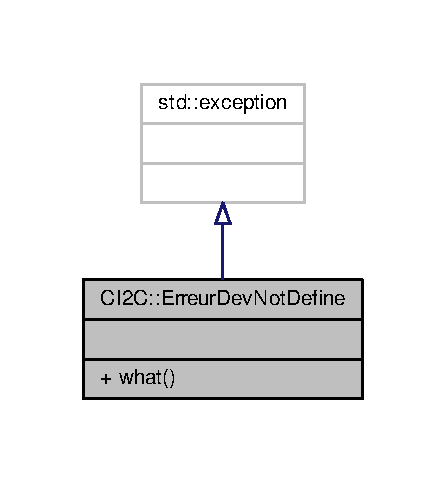
\includegraphics[width=214pt]{classCI2C_1_1ErreurDevNotDefine__inherit__graph}
\end{center}
\end{figure}


Graphe de collaboration de C\+I2\+C\+:\+:Erreur\+Dev\+Not\+Define\+:\nopagebreak
\begin{figure}[H]
\begin{center}
\leavevmode
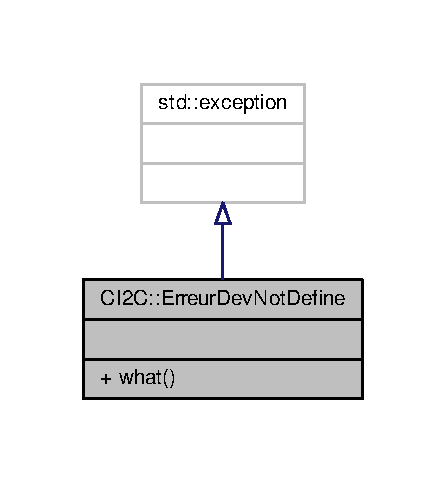
\includegraphics[width=214pt]{classCI2C_1_1ErreurDevNotDefine__coll__graph}
\end{center}
\end{figure}
\subsection*{Fonctions membres publiques}
\begin{DoxyCompactItemize}
\item 
virtual const char $\ast$ \hyperlink{classCI2C_1_1ErreurDevNotDefine_a8c2f805ea7adc632db53c58437c2884e}{what} () const noexcept
\begin{DoxyCompactList}\small\item\em Methode what. \end{DoxyCompactList}\end{DoxyCompactItemize}


\subsection{Description détaillée}
exception device non défini 

\subsection{Documentation des fonctions membres}
\hypertarget{classCI2C_1_1ErreurDevNotDefine_a8c2f805ea7adc632db53c58437c2884e}{\index{C\+I2\+C\+::\+Erreur\+Dev\+Not\+Define@{C\+I2\+C\+::\+Erreur\+Dev\+Not\+Define}!what@{what}}
\index{what@{what}!C\+I2\+C\+::\+Erreur\+Dev\+Not\+Define@{C\+I2\+C\+::\+Erreur\+Dev\+Not\+Define}}
\subsubsection[{what}]{\setlength{\rightskip}{0pt plus 5cm}virtual const char$\ast$ C\+I2\+C\+::\+Erreur\+Dev\+Not\+Define\+::what (
\begin{DoxyParamCaption}
{}
\end{DoxyParamCaption}
) const\hspace{0.3cm}{\ttfamily [inline]}, {\ttfamily [virtual]}, {\ttfamily [noexcept]}}}\label{classCI2C_1_1ErreurDevNotDefine_a8c2f805ea7adc632db53c58437c2884e}


Methode what. 

\begin{DoxyReturn}{Renvoie}
la description de l'exception 
\end{DoxyReturn}


La documentation de cette classe a été générée à partir du fichier suivant \+:\begin{DoxyCompactItemize}
\item 
/home/jam/\+Bureau/\+C++/\+Classes/\+C\+I2\+C/\hyperlink{CI2C_8h}{C\+I2\+C.\+h}\end{DoxyCompactItemize}

\hypertarget{classCI2C_1_1ErreurOpenDev}{\section{Référence de la classe C\+I2\+C\+:\+:Erreur\+Open\+Dev}
\label{classCI2C_1_1ErreurOpenDev}\index{C\+I2\+C\+::\+Erreur\+Open\+Dev@{C\+I2\+C\+::\+Erreur\+Open\+Dev}}
}


exception lorsqu'on essaye d'ouvrir le dev spécifié  




{\ttfamily \#include $<$C\+I2\+C.\+h$>$}



Graphe d'héritage de C\+I2\+C\+:\+:Erreur\+Open\+Dev\+:\nopagebreak
\begin{figure}[H]
\begin{center}
\leavevmode
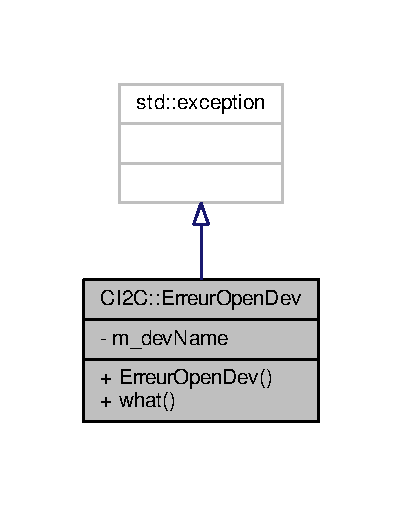
\includegraphics[width=193pt]{classCI2C_1_1ErreurOpenDev__inherit__graph}
\end{center}
\end{figure}


Graphe de collaboration de C\+I2\+C\+:\+:Erreur\+Open\+Dev\+:\nopagebreak
\begin{figure}[H]
\begin{center}
\leavevmode
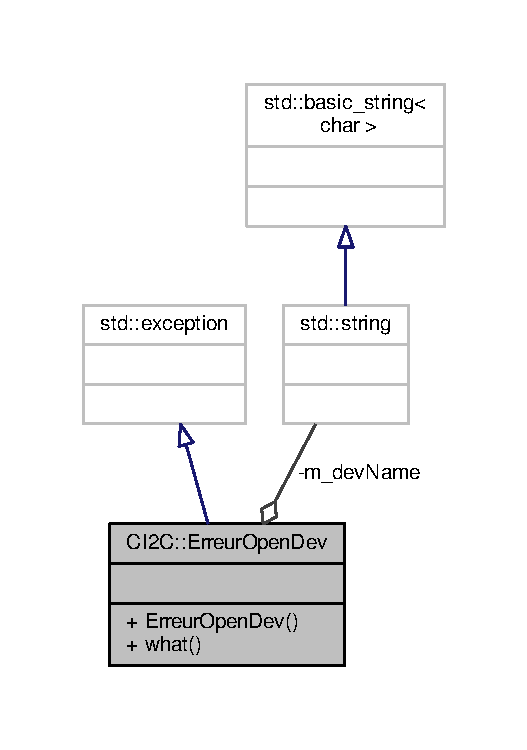
\includegraphics[width=253pt]{classCI2C_1_1ErreurOpenDev__coll__graph}
\end{center}
\end{figure}
\subsection*{Fonctions membres publiques}
\begin{DoxyCompactItemize}
\item 
\hyperlink{classCI2C_1_1ErreurOpenDev_ac741480179a06b9d23f4c5c49500a5e1}{Erreur\+Open\+Dev} (string dev\+Name)
\begin{DoxyCompactList}\small\item\em Contructeur de la classe \hyperlink{classCI2C_1_1ErreurOpenDev}{Erreur\+Open\+Dev}. \end{DoxyCompactList}\item 
virtual const char $\ast$ \hyperlink{classCI2C_1_1ErreurOpenDev_a52441e7b0de2a74dd51c67504bb93fe1}{what} () const noexcept
\begin{DoxyCompactList}\small\item\em Methode what. \end{DoxyCompactList}\end{DoxyCompactItemize}
\subsection*{Attributs privés}
\begin{DoxyCompactItemize}
\item 
\hypertarget{classCI2C_1_1ErreurOpenDev_a19fcf1034384789940c900e32953e857}{string \hyperlink{classCI2C_1_1ErreurOpenDev_a19fcf1034384789940c900e32953e857}{m\+\_\+dev\+Name}}\label{classCI2C_1_1ErreurOpenDev_a19fcf1034384789940c900e32953e857}

\begin{DoxyCompactList}\small\item\em contient le nom du device que l'on essaye d'ouvrir \end{DoxyCompactList}\end{DoxyCompactItemize}


\subsection{Description détaillée}
exception lorsqu'on essaye d'ouvrir le dev spécifié 

\subsection{Documentation des constructeurs et destructeur}
\hypertarget{classCI2C_1_1ErreurOpenDev_ac741480179a06b9d23f4c5c49500a5e1}{\index{C\+I2\+C\+::\+Erreur\+Open\+Dev@{C\+I2\+C\+::\+Erreur\+Open\+Dev}!Erreur\+Open\+Dev@{Erreur\+Open\+Dev}}
\index{Erreur\+Open\+Dev@{Erreur\+Open\+Dev}!C\+I2\+C\+::\+Erreur\+Open\+Dev@{C\+I2\+C\+::\+Erreur\+Open\+Dev}}
\subsubsection[{Erreur\+Open\+Dev}]{\setlength{\rightskip}{0pt plus 5cm}C\+I2\+C\+::\+Erreur\+Open\+Dev\+::\+Erreur\+Open\+Dev (
\begin{DoxyParamCaption}
\item[{string}]{dev\+Name}
\end{DoxyParamCaption}
)\hspace{0.3cm}{\ttfamily [inline]}}}\label{classCI2C_1_1ErreurOpenDev_ac741480179a06b9d23f4c5c49500a5e1}


Contructeur de la classe \hyperlink{classCI2C_1_1ErreurOpenDev}{Erreur\+Open\+Dev}. 

Ce contructeur initialise les attributs de la classe \hyperlink{classCI2C_1_1ErreurOpenDev}{Erreur\+Open\+Dev}


\begin{DoxyParams}[1]{Paramètres}
\mbox{\tt in}  & {\em dev\+Name} & \+: le nom du device que l'on a essayé d'ouvrir \\
\hline
\end{DoxyParams}


\subsection{Documentation des fonctions membres}
\hypertarget{classCI2C_1_1ErreurOpenDev_a52441e7b0de2a74dd51c67504bb93fe1}{\index{C\+I2\+C\+::\+Erreur\+Open\+Dev@{C\+I2\+C\+::\+Erreur\+Open\+Dev}!what@{what}}
\index{what@{what}!C\+I2\+C\+::\+Erreur\+Open\+Dev@{C\+I2\+C\+::\+Erreur\+Open\+Dev}}
\subsubsection[{what}]{\setlength{\rightskip}{0pt plus 5cm}virtual const char$\ast$ C\+I2\+C\+::\+Erreur\+Open\+Dev\+::what (
\begin{DoxyParamCaption}
{}
\end{DoxyParamCaption}
) const\hspace{0.3cm}{\ttfamily [inline]}, {\ttfamily [virtual]}, {\ttfamily [noexcept]}}}\label{classCI2C_1_1ErreurOpenDev_a52441e7b0de2a74dd51c67504bb93fe1}


Methode what. 

\begin{DoxyReturn}{Renvoie}
la description de l'exception avec le nom du device que l'on a essayé d'ouvrir 
\end{DoxyReturn}


La documentation de cette classe a été générée à partir du fichier suivant \+:\begin{DoxyCompactItemize}
\item 
/home/jam/\+Bureau/\+C++/\+Classes/\+C\+I2\+C/\hyperlink{CI2C_8h}{C\+I2\+C.\+h}\end{DoxyCompactItemize}

\hypertarget{classCI2C_1_1ErreurRead}{\section{Référence de la classe C\+I2\+C\+:\+:Erreur\+Read}
\label{classCI2C_1_1ErreurRead}\index{C\+I2\+C\+::\+Erreur\+Read@{C\+I2\+C\+::\+Erreur\+Read}}
}


Cette classe est une exception qui est levé lorsqu'il y a un erreur de lecture.  




{\ttfamily \#include $<$C\+I2\+C.\+h$>$}



Graphe d'héritage de C\+I2\+C\+:\+:Erreur\+Read\+:\nopagebreak
\begin{figure}[H]
\begin{center}
\leavevmode
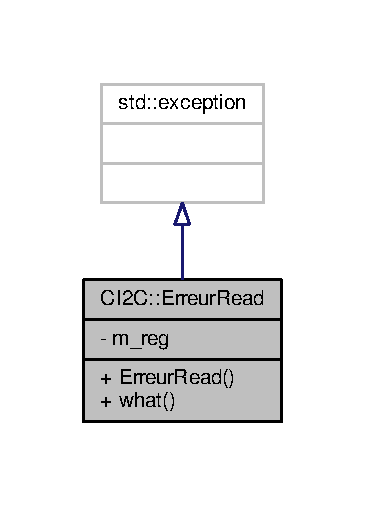
\includegraphics[width=175pt]{classCI2C_1_1ErreurRead__inherit__graph}
\end{center}
\end{figure}


Graphe de collaboration de C\+I2\+C\+:\+:Erreur\+Read\+:\nopagebreak
\begin{figure}[H]
\begin{center}
\leavevmode
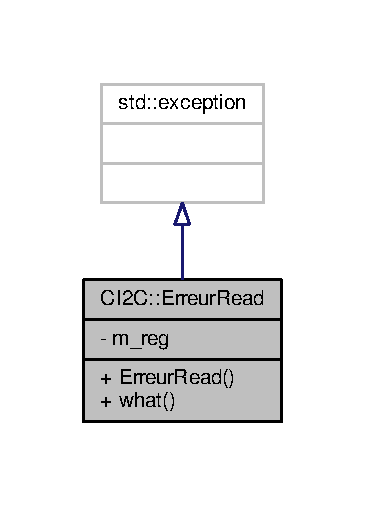
\includegraphics[width=175pt]{classCI2C_1_1ErreurRead__coll__graph}
\end{center}
\end{figure}
\subsection*{Fonctions membres publiques}
\begin{DoxyCompactItemize}
\item 
\hyperlink{classCI2C_1_1ErreurRead_a2006046ac1989f7d8f36e73365a7430d}{Erreur\+Read} (int reg)
\begin{DoxyCompactList}\small\item\em Constructeur de la classe \hyperlink{classCI2C_1_1ErreurRead}{Erreur\+Read}. \end{DoxyCompactList}\item 
virtual const char $\ast$ \hyperlink{classCI2C_1_1ErreurRead_a43289e1f3f662de4ee81036a98b2ed55}{what} () const noexcept
\begin{DoxyCompactList}\small\item\em Methode what. \end{DoxyCompactList}\end{DoxyCompactItemize}
\subsection*{Attributs privés}
\begin{DoxyCompactItemize}
\item 
\hypertarget{classCI2C_1_1ErreurRead_a8af2c5a4b9b952aa97537fd2c59745a5}{int \hyperlink{classCI2C_1_1ErreurRead_a8af2c5a4b9b952aa97537fd2c59745a5}{m\+\_\+reg}}\label{classCI2C_1_1ErreurRead_a8af2c5a4b9b952aa97537fd2c59745a5}

\begin{DoxyCompactList}\small\item\em Contient le registre que l'on a essayé de lire. \end{DoxyCompactList}\end{DoxyCompactItemize}


\subsection{Description détaillée}
Cette classe est une exception qui est levé lorsqu'il y a un erreur de lecture. 

\subsection{Documentation des constructeurs et destructeur}
\hypertarget{classCI2C_1_1ErreurRead_a2006046ac1989f7d8f36e73365a7430d}{\index{C\+I2\+C\+::\+Erreur\+Read@{C\+I2\+C\+::\+Erreur\+Read}!Erreur\+Read@{Erreur\+Read}}
\index{Erreur\+Read@{Erreur\+Read}!C\+I2\+C\+::\+Erreur\+Read@{C\+I2\+C\+::\+Erreur\+Read}}
\subsubsection[{Erreur\+Read}]{\setlength{\rightskip}{0pt plus 5cm}C\+I2\+C\+::\+Erreur\+Read\+::\+Erreur\+Read (
\begin{DoxyParamCaption}
\item[{int}]{reg}
\end{DoxyParamCaption}
)\hspace{0.3cm}{\ttfamily [inline]}}}\label{classCI2C_1_1ErreurRead_a2006046ac1989f7d8f36e73365a7430d}


Constructeur de la classe \hyperlink{classCI2C_1_1ErreurRead}{Erreur\+Read}. 

Ce contructeur initialise les attributs de la classe \hyperlink{classCI2C_1_1ErreurWrite}{Erreur\+Write}


\begin{DoxyParams}[1]{Paramètres}
\mbox{\tt in}  & {\em reg} & \+: le registre que l'on a essayé de lire \\
\hline
\end{DoxyParams}


\subsection{Documentation des fonctions membres}
\hypertarget{classCI2C_1_1ErreurRead_a43289e1f3f662de4ee81036a98b2ed55}{\index{C\+I2\+C\+::\+Erreur\+Read@{C\+I2\+C\+::\+Erreur\+Read}!what@{what}}
\index{what@{what}!C\+I2\+C\+::\+Erreur\+Read@{C\+I2\+C\+::\+Erreur\+Read}}
\subsubsection[{what}]{\setlength{\rightskip}{0pt plus 5cm}virtual const char$\ast$ C\+I2\+C\+::\+Erreur\+Read\+::what (
\begin{DoxyParamCaption}
{}
\end{DoxyParamCaption}
) const\hspace{0.3cm}{\ttfamily [inline]}, {\ttfamily [virtual]}, {\ttfamily [noexcept]}}}\label{classCI2C_1_1ErreurRead_a43289e1f3f662de4ee81036a98b2ed55}


Methode what. 

\begin{DoxyReturn}{Renvoie}
la description de l'esception avec la valeur du registre que l'on a essayé de lire 
\end{DoxyReturn}


La documentation de cette classe a été générée à partir du fichier suivant \+:\begin{DoxyCompactItemize}
\item 
/home/jam/\+Bureau/\+C++/\+Classes/\+C\+I2\+C/\hyperlink{CI2C_8h}{C\+I2\+C.\+h}\end{DoxyCompactItemize}

\hypertarget{classCI2C_1_1ErreurSetAddrSlave}{\section{Référence de la classe C\+I2\+C\+:\+:Erreur\+Set\+Addr\+Slave}
\label{classCI2C_1_1ErreurSetAddrSlave}\index{C\+I2\+C\+::\+Erreur\+Set\+Addr\+Slave@{C\+I2\+C\+::\+Erreur\+Set\+Addr\+Slave}}
}


exception definition de l'esclave  




{\ttfamily \#include $<$C\+I2\+C.\+h$>$}



Graphe d'héritage de C\+I2\+C\+:\+:Erreur\+Set\+Addr\+Slave\+:\nopagebreak
\begin{figure}[H]
\begin{center}
\leavevmode
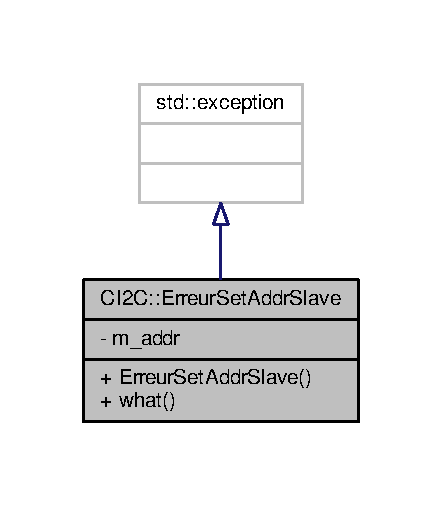
\includegraphics[width=212pt]{classCI2C_1_1ErreurSetAddrSlave__inherit__graph}
\end{center}
\end{figure}


Graphe de collaboration de C\+I2\+C\+:\+:Erreur\+Set\+Addr\+Slave\+:\nopagebreak
\begin{figure}[H]
\begin{center}
\leavevmode
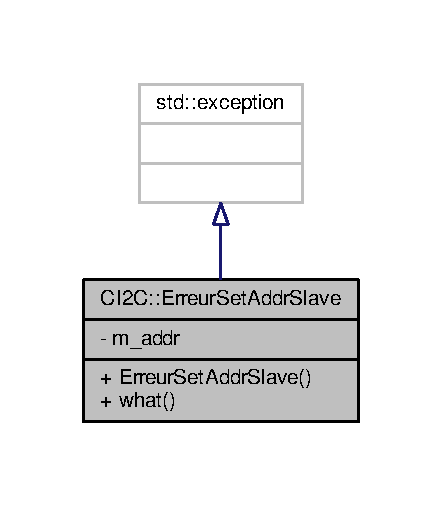
\includegraphics[width=212pt]{classCI2C_1_1ErreurSetAddrSlave__coll__graph}
\end{center}
\end{figure}
\subsection*{Fonctions membres publiques}
\begin{DoxyCompactItemize}
\item 
\hyperlink{classCI2C_1_1ErreurSetAddrSlave_ac92f34eb7c68e1b29ae55e0b147bdc02}{Erreur\+Set\+Addr\+Slave} (int addr)
\begin{DoxyCompactList}\small\item\em Constructeur de la classe \hyperlink{classCI2C_1_1ErreurSetAddrSlave}{Erreur\+Set\+Addr\+Slave}. \end{DoxyCompactList}\item 
virtual const char $\ast$ \hyperlink{classCI2C_1_1ErreurSetAddrSlave_a6f82e7fa42f2ea5bb39d9c06517c5b09}{what} () const noexcept
\begin{DoxyCompactList}\small\item\em Methode what. \end{DoxyCompactList}\end{DoxyCompactItemize}
\subsection*{Attributs privés}
\begin{DoxyCompactItemize}
\item 
\hypertarget{classCI2C_1_1ErreurSetAddrSlave_aebf96cc2020fd45215280d41648151d8}{int \hyperlink{classCI2C_1_1ErreurSetAddrSlave_aebf96cc2020fd45215280d41648151d8}{m\+\_\+addr}}\label{classCI2C_1_1ErreurSetAddrSlave_aebf96cc2020fd45215280d41648151d8}

\begin{DoxyCompactList}\small\item\em Contient l'addresse de l'esclave avec lequel on veux communiquer. \end{DoxyCompactList}\end{DoxyCompactItemize}


\subsection{Description détaillée}
exception definition de l'esclave 

\subsection{Documentation des constructeurs et destructeur}
\hypertarget{classCI2C_1_1ErreurSetAddrSlave_ac92f34eb7c68e1b29ae55e0b147bdc02}{\index{C\+I2\+C\+::\+Erreur\+Set\+Addr\+Slave@{C\+I2\+C\+::\+Erreur\+Set\+Addr\+Slave}!Erreur\+Set\+Addr\+Slave@{Erreur\+Set\+Addr\+Slave}}
\index{Erreur\+Set\+Addr\+Slave@{Erreur\+Set\+Addr\+Slave}!C\+I2\+C\+::\+Erreur\+Set\+Addr\+Slave@{C\+I2\+C\+::\+Erreur\+Set\+Addr\+Slave}}
\subsubsection[{Erreur\+Set\+Addr\+Slave}]{\setlength{\rightskip}{0pt plus 5cm}C\+I2\+C\+::\+Erreur\+Set\+Addr\+Slave\+::\+Erreur\+Set\+Addr\+Slave (
\begin{DoxyParamCaption}
\item[{int}]{addr}
\end{DoxyParamCaption}
)\hspace{0.3cm}{\ttfamily [inline]}}}\label{classCI2C_1_1ErreurSetAddrSlave_ac92f34eb7c68e1b29ae55e0b147bdc02}


Constructeur de la classe \hyperlink{classCI2C_1_1ErreurSetAddrSlave}{Erreur\+Set\+Addr\+Slave}. 

Ce contructeur initialise les attributs de la classe \hyperlink{classCI2C_1_1ErreurSetAddrSlave}{Erreur\+Set\+Addr\+Slave}


\begin{DoxyParams}[1]{Paramètres}
\mbox{\tt in}  & {\em addr} & \+: l'adresse de l'esclave avec lequel on veux communiquer \\
\hline
\end{DoxyParams}


\subsection{Documentation des fonctions membres}
\hypertarget{classCI2C_1_1ErreurSetAddrSlave_a6f82e7fa42f2ea5bb39d9c06517c5b09}{\index{C\+I2\+C\+::\+Erreur\+Set\+Addr\+Slave@{C\+I2\+C\+::\+Erreur\+Set\+Addr\+Slave}!what@{what}}
\index{what@{what}!C\+I2\+C\+::\+Erreur\+Set\+Addr\+Slave@{C\+I2\+C\+::\+Erreur\+Set\+Addr\+Slave}}
\subsubsection[{what}]{\setlength{\rightskip}{0pt plus 5cm}virtual const char$\ast$ C\+I2\+C\+::\+Erreur\+Set\+Addr\+Slave\+::what (
\begin{DoxyParamCaption}
{}
\end{DoxyParamCaption}
) const\hspace{0.3cm}{\ttfamily [inline]}, {\ttfamily [virtual]}, {\ttfamily [noexcept]}}}\label{classCI2C_1_1ErreurSetAddrSlave_a6f82e7fa42f2ea5bb39d9c06517c5b09}


Methode what. 

\begin{DoxyReturn}{Renvoie}
la description de l'exception 
\end{DoxyReturn}


La documentation de cette classe a été générée à partir du fichier suivant \+:\begin{DoxyCompactItemize}
\item 
/home/jam/\+Bureau/\+C++/\+Classes/\+C\+I2\+C/\hyperlink{CI2C_8h}{C\+I2\+C.\+h}\end{DoxyCompactItemize}

\hypertarget{classCI2C_1_1ErreurSlaveNotDefine}{\section{Référence de la classe C\+I2\+C\+:\+:Erreur\+Slave\+Not\+Define}
\label{classCI2C_1_1ErreurSlaveNotDefine}\index{C\+I2\+C\+::\+Erreur\+Slave\+Not\+Define@{C\+I2\+C\+::\+Erreur\+Slave\+Not\+Define}}
}


exception adresse de l'esclave non défini  




{\ttfamily \#include $<$C\+I2\+C.\+h$>$}



Graphe d'héritage de C\+I2\+C\+:\+:Erreur\+Slave\+Not\+Define\+:\nopagebreak
\begin{figure}[H]
\begin{center}
\leavevmode
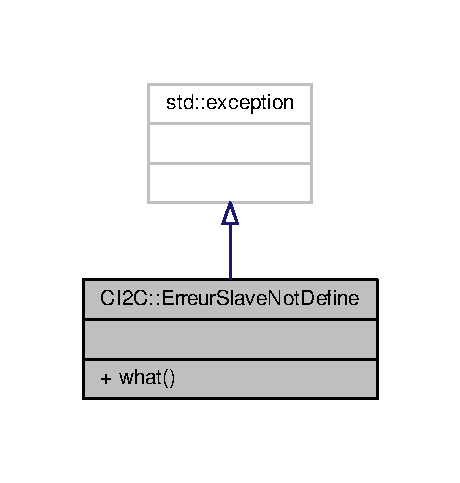
\includegraphics[width=221pt]{classCI2C_1_1ErreurSlaveNotDefine__inherit__graph}
\end{center}
\end{figure}


Graphe de collaboration de C\+I2\+C\+:\+:Erreur\+Slave\+Not\+Define\+:\nopagebreak
\begin{figure}[H]
\begin{center}
\leavevmode
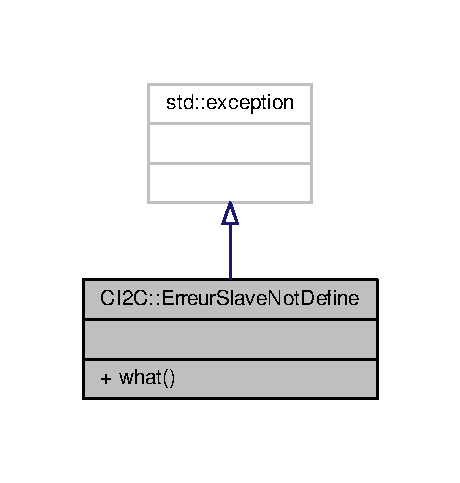
\includegraphics[width=221pt]{classCI2C_1_1ErreurSlaveNotDefine__coll__graph}
\end{center}
\end{figure}
\subsection*{Fonctions membres publiques}
\begin{DoxyCompactItemize}
\item 
virtual const char $\ast$ \hyperlink{classCI2C_1_1ErreurSlaveNotDefine_a7efd5525f6598a091e21519cfcc3cd95}{what} () const noexcept
\begin{DoxyCompactList}\small\item\em Methode what. \end{DoxyCompactList}\end{DoxyCompactItemize}


\subsection{Description détaillée}
exception adresse de l'esclave non défini 

\subsection{Documentation des fonctions membres}
\hypertarget{classCI2C_1_1ErreurSlaveNotDefine_a7efd5525f6598a091e21519cfcc3cd95}{\index{C\+I2\+C\+::\+Erreur\+Slave\+Not\+Define@{C\+I2\+C\+::\+Erreur\+Slave\+Not\+Define}!what@{what}}
\index{what@{what}!C\+I2\+C\+::\+Erreur\+Slave\+Not\+Define@{C\+I2\+C\+::\+Erreur\+Slave\+Not\+Define}}
\subsubsection[{what}]{\setlength{\rightskip}{0pt plus 5cm}virtual const char$\ast$ C\+I2\+C\+::\+Erreur\+Slave\+Not\+Define\+::what (
\begin{DoxyParamCaption}
{}
\end{DoxyParamCaption}
) const\hspace{0.3cm}{\ttfamily [inline]}, {\ttfamily [virtual]}, {\ttfamily [noexcept]}}}\label{classCI2C_1_1ErreurSlaveNotDefine_a7efd5525f6598a091e21519cfcc3cd95}


Methode what. 

\begin{DoxyReturn}{Renvoie}
la description de l'exception 
\end{DoxyReturn}


La documentation de cette classe a été générée à partir du fichier suivant \+:\begin{DoxyCompactItemize}
\item 
/home/jam/\+Bureau/\+C++/\+Classes/\+C\+I2\+C/\hyperlink{CI2C_8h}{C\+I2\+C.\+h}\end{DoxyCompactItemize}

\hypertarget{classCI2C_1_1ErreurWrite}{\section{Référence de la classe C\+I2\+C\+:\+:Erreur\+Write}
\label{classCI2C_1_1ErreurWrite}\index{C\+I2\+C\+::\+Erreur\+Write@{C\+I2\+C\+::\+Erreur\+Write}}
}


Cette classe est une esception qui est levé lorsqu'il y a une erreur d'écriture.  




{\ttfamily \#include $<$C\+I2\+C.\+h$>$}



Graphe d'héritage de C\+I2\+C\+:\+:Erreur\+Write\+:\nopagebreak
\begin{figure}[H]
\begin{center}
\leavevmode
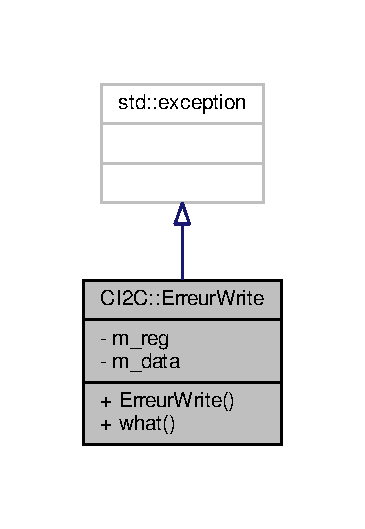
\includegraphics[width=175pt]{classCI2C_1_1ErreurWrite__inherit__graph}
\end{center}
\end{figure}


Graphe de collaboration de C\+I2\+C\+:\+:Erreur\+Write\+:\nopagebreak
\begin{figure}[H]
\begin{center}
\leavevmode
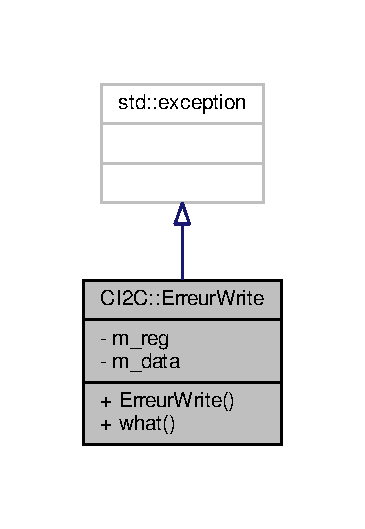
\includegraphics[width=175pt]{classCI2C_1_1ErreurWrite__coll__graph}
\end{center}
\end{figure}
\subsection*{Fonctions membres publiques}
\begin{DoxyCompactItemize}
\item 
\hyperlink{classCI2C_1_1ErreurWrite_a8d3b2f6b46d6bb5e4b26e5fdce8e80b4}{Erreur\+Write} (int reg, int data)
\begin{DoxyCompactList}\small\item\em Constructeur de la classe \hyperlink{classCI2C_1_1ErreurWrite}{Erreur\+Write}. \end{DoxyCompactList}\item 
virtual const char $\ast$ \hyperlink{classCI2C_1_1ErreurWrite_ad76aa069d233146923c4a244d2da9665}{what} () const noexcept
\begin{DoxyCompactList}\small\item\em Methode what. \end{DoxyCompactList}\end{DoxyCompactItemize}
\subsection*{Attributs privés}
\begin{DoxyCompactItemize}
\item 
\hypertarget{classCI2C_1_1ErreurWrite_a0271678b0343dd18ad8113ab3dd579d2}{int \hyperlink{classCI2C_1_1ErreurWrite_a0271678b0343dd18ad8113ab3dd579d2}{m\+\_\+reg}}\label{classCI2C_1_1ErreurWrite_a0271678b0343dd18ad8113ab3dd579d2}

\begin{DoxyCompactList}\small\item\em Contient le registre dans lequel on a essayé d'écrire. \end{DoxyCompactList}\item 
\hypertarget{classCI2C_1_1ErreurWrite_a3ba1d239d00892177274b494e987862b}{int \hyperlink{classCI2C_1_1ErreurWrite_a3ba1d239d00892177274b494e987862b}{m\+\_\+data}}\label{classCI2C_1_1ErreurWrite_a3ba1d239d00892177274b494e987862b}

\begin{DoxyCompactList}\small\item\em Contient la valeur qu'on a essayer d'écrire dans le registre. \end{DoxyCompactList}\end{DoxyCompactItemize}


\subsection{Description détaillée}
Cette classe est une esception qui est levé lorsqu'il y a une erreur d'écriture. 

\subsection{Documentation des constructeurs et destructeur}
\hypertarget{classCI2C_1_1ErreurWrite_a8d3b2f6b46d6bb5e4b26e5fdce8e80b4}{\index{C\+I2\+C\+::\+Erreur\+Write@{C\+I2\+C\+::\+Erreur\+Write}!Erreur\+Write@{Erreur\+Write}}
\index{Erreur\+Write@{Erreur\+Write}!C\+I2\+C\+::\+Erreur\+Write@{C\+I2\+C\+::\+Erreur\+Write}}
\subsubsection[{Erreur\+Write}]{\setlength{\rightskip}{0pt plus 5cm}C\+I2\+C\+::\+Erreur\+Write\+::\+Erreur\+Write (
\begin{DoxyParamCaption}
\item[{int}]{reg, }
\item[{int}]{data}
\end{DoxyParamCaption}
)\hspace{0.3cm}{\ttfamily [inline]}}}\label{classCI2C_1_1ErreurWrite_a8d3b2f6b46d6bb5e4b26e5fdce8e80b4}


Constructeur de la classe \hyperlink{classCI2C_1_1ErreurWrite}{Erreur\+Write}. 

Ce contructeur initialise les attributs de la classe \hyperlink{classCI2C_1_1ErreurWrite}{Erreur\+Write}


\begin{DoxyParams}[1]{Paramètres}
\mbox{\tt in}  & {\em reg} & \+: le registre dans lequel on essaye d'écrire \\
\hline
\mbox{\tt in}  & {\em data} & \+: la valeur que l'on essaye d'écrire dans le registre \\
\hline
\end{DoxyParams}


\subsection{Documentation des fonctions membres}
\hypertarget{classCI2C_1_1ErreurWrite_ad76aa069d233146923c4a244d2da9665}{\index{C\+I2\+C\+::\+Erreur\+Write@{C\+I2\+C\+::\+Erreur\+Write}!what@{what}}
\index{what@{what}!C\+I2\+C\+::\+Erreur\+Write@{C\+I2\+C\+::\+Erreur\+Write}}
\subsubsection[{what}]{\setlength{\rightskip}{0pt plus 5cm}virtual const char$\ast$ C\+I2\+C\+::\+Erreur\+Write\+::what (
\begin{DoxyParamCaption}
{}
\end{DoxyParamCaption}
) const\hspace{0.3cm}{\ttfamily [inline]}, {\ttfamily [virtual]}, {\ttfamily [noexcept]}}}\label{classCI2C_1_1ErreurWrite_ad76aa069d233146923c4a244d2da9665}


Methode what. 

\begin{DoxyReturn}{Renvoie}
la description de l'exception avec la valeur et le registre qui ont provoqué l'erreur 
\end{DoxyReturn}


La documentation de cette classe a été générée à partir du fichier suivant \+:\begin{DoxyCompactItemize}
\item 
/home/jam/\+Bureau/\+C++/\+Classes/\+C\+I2\+C/\hyperlink{CI2C_8h}{C\+I2\+C.\+h}\end{DoxyCompactItemize}

\chapter{Documentation des fichiers}
\hypertarget{CI2C_8cpp}{\section{Référence du fichier /home/jam/\+Bureau/\+C++/\+Classes/\+C\+I2\+C/\+C\+I2\+C.cpp}
\label{CI2C_8cpp}\index{/home/jam/\+Bureau/\+C++/\+Classes/\+C\+I2\+C/\+C\+I2\+C.\+cpp@{/home/jam/\+Bureau/\+C++/\+Classes/\+C\+I2\+C/\+C\+I2\+C.\+cpp}}
}


Contient la définition de la classe \hyperlink{classCI2C}{C\+I2\+C}.  


{\ttfamily \#include \char`\"{}C\+I2\+C.\+h\char`\"{}}\\*
Graphe des dépendances par inclusion de C\+I2\+C.\+cpp\+:\nopagebreak
\begin{figure}[H]
\begin{center}
\leavevmode
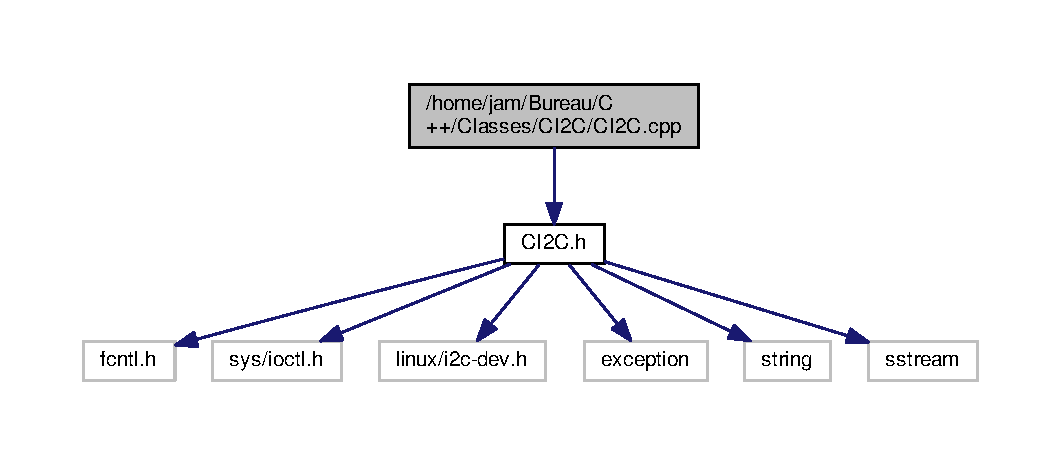
\includegraphics[width=350pt]{CI2C_8cpp__incl}
\end{center}
\end{figure}


\subsection{Description détaillée}
Contient la définition de la classe \hyperlink{classCI2C}{C\+I2\+C}. 


\hypertarget{CI2C_8h}{\section{Référence du fichier /home/jam/\+Bureau/\+C++/\+Classes/\+C\+I2\+C/\+C\+I2\+C.h}
\label{CI2C_8h}\index{/home/jam/\+Bureau/\+C++/\+Classes/\+C\+I2\+C/\+C\+I2\+C.\+h@{/home/jam/\+Bureau/\+C++/\+Classes/\+C\+I2\+C/\+C\+I2\+C.\+h}}
}


Contient la declaration de la \hyperlink{classCI2C}{C\+I2\+C}.  


{\ttfamily \#include $<$fcntl.\+h$>$}\\*
{\ttfamily \#include $<$sys/ioctl.\+h$>$}\\*
{\ttfamily \#include $<$linux/i2c-\/dev.\+h$>$}\\*
{\ttfamily \#include $<$exception$>$}\\*
{\ttfamily \#include $<$string$>$}\\*
{\ttfamily \#include $<$sstream$>$}\\*
Graphe des dépendances par inclusion de C\+I2\+C.\+h\+:\nopagebreak
\begin{figure}[H]
\begin{center}
\leavevmode
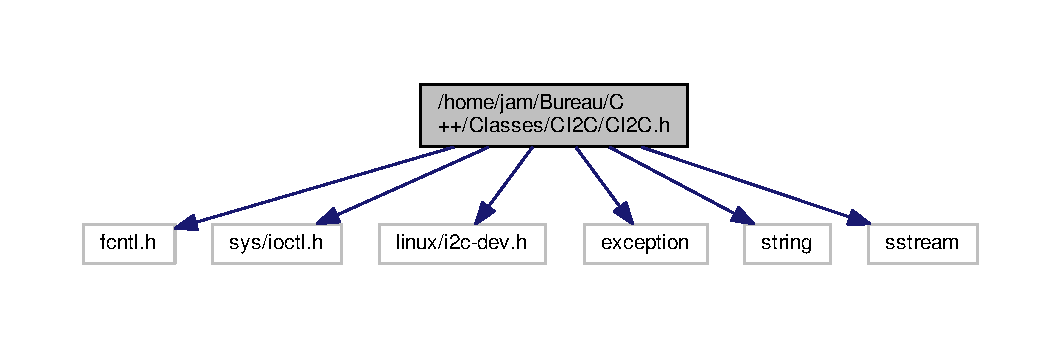
\includegraphics[width=350pt]{CI2C_8h__incl}
\end{center}
\end{figure}
Ce graphe montre quels fichiers incluent directement ou indirectement ce fichier \+:\nopagebreak
\begin{figure}[H]
\begin{center}
\leavevmode
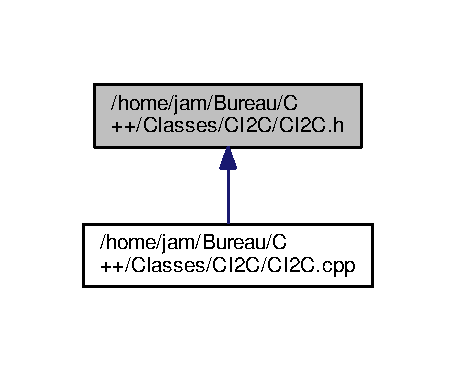
\includegraphics[width=219pt]{CI2C_8h__dep__incl}
\end{center}
\end{figure}
\subsection*{Classes}
\begin{DoxyCompactItemize}
\item 
class \hyperlink{classCI2C}{C\+I2\+C}
\begin{DoxyCompactList}\small\item\em Cette classe \hyperlink{classCI2C}{C\+I2\+C} permet de lire/écrire les valeurs de registres des esclaves d'un bus I2\+C. \end{DoxyCompactList}\item 
class \hyperlink{classCI2C_1_1ErreurWrite}{C\+I2\+C\+::\+Erreur\+Write}
\begin{DoxyCompactList}\small\item\em Cette classe est une esception qui est levé lorsqu'il y a une erreur d'écriture. \end{DoxyCompactList}\item 
class \hyperlink{classCI2C_1_1ErreurRead}{C\+I2\+C\+::\+Erreur\+Read}
\begin{DoxyCompactList}\small\item\em Cette classe est une exception qui est levé lorsqu'il y a un erreur de lecture. \end{DoxyCompactList}\item 
class \hyperlink{classCI2C_1_1ErreurOpenDev}{C\+I2\+C\+::\+Erreur\+Open\+Dev}
\begin{DoxyCompactList}\small\item\em exception lorsqu'on essaye d'ouvrir le dev spécifié \end{DoxyCompactList}\item 
class \hyperlink{classCI2C_1_1ErreurSetAddrSlave}{C\+I2\+C\+::\+Erreur\+Set\+Addr\+Slave}
\begin{DoxyCompactList}\small\item\em exception definition de l'esclave \end{DoxyCompactList}\item 
class \hyperlink{classCI2C_1_1ErreurDevNotDefine}{C\+I2\+C\+::\+Erreur\+Dev\+Not\+Define}
\begin{DoxyCompactList}\small\item\em exception device non défini \end{DoxyCompactList}\item 
class \hyperlink{classCI2C_1_1ErreurSlaveNotDefine}{C\+I2\+C\+::\+Erreur\+Slave\+Not\+Define}
\begin{DoxyCompactList}\small\item\em exception adresse de l'esclave non défini \end{DoxyCompactList}\end{DoxyCompactItemize}
\subsection*{Macros}
\begin{DoxyCompactItemize}
\item 
\hypertarget{CI2C_8h_ab15137f7c592d05573de99f078516157}{\#define {\bfseries I2\+C\+\_\+\+S\+L\+A\+V\+E}~0x0703}\label{CI2C_8h_ab15137f7c592d05573de99f078516157}

\end{DoxyCompactItemize}


\subsection{Description détaillée}
Contient la declaration de la \hyperlink{classCI2C}{C\+I2\+C}. 


%--- End generated contents ---

% Index
\newpage
\phantomsection
\addcontentsline{toc}{chapter}{Index}
\printindex

\end{document}
